
\providecommand{\Cat}{\mathcal{C}at}
\providecommand{\hTwoCell}[5]{\tikz[baseline=-0.8ex]{%
  \node (rvl) at (0,0) {$#1$};
  \node (rvr) at (2.9,0) {$#2$};
  \draw[->] (rvl) to[bend left=28] node[above]{$\scriptstyle #3$} (rvr);
  \draw[->] (rvl) to[bend right=28] node[below]{$\scriptstyle #5$} (rvr);
  \node at (1.45,0) {$\scriptstyle #4$};}}

\section{2-\trCategory{}的 3-\trCategory}\label{sec:the-3-category-of-2-categories}

通常的 1-\trCategory{}构成一个由\trCategory、\trFunctor{}与%
\trNaturalTransformation{}组成的 2-\trCategory{}的对象。类似地，2-\trCategory{}%
构成一个由 2-\trCategory、2-\trFunctor、2-\trNaturalTransformation{}与\trModification{}组成
的 3-\trCategory{}的对象。在本节中，我们将简要地介绍所有这些概念。

回忆\cref{def:two-category}：一个 2-\trCategory{}是富集于 $\Cat$ 之上的一个\trCategory。
类似地，2-\trFunctor{}与 2-\trNaturalTransformation{}恰是附录 A 中的那些
$\Cat$-富集\trFunctor{}与 $\Cat$-富集\trNaturalTransformation。由附录 A 中的%
\cref{cor:vcat-two-category}，2-\trCategory、2-\trFunctor{}与
2-\trNaturalTransformation{}拼装成一个 2-\trCategory。2-\trCategory{}之间的
$3$ 维\trCell{}——即诸\trModification{}——是利用一个 2-\trCategory{}的 2-\trCell{}来定义
的，正如 1-\trCategory{}之间的 $2$ 维\trCell{}——即诸\trNaturalTransformation{}——%
是利用一个 1-\trCategory{}中的 1-\trCell{}来定义的一样。

\begin{definition}\label{def:two-functor}
介于 2-\trCategory{}之间的一个\textbf{\trTwoFunctor}
$F\colon\mathcal{C}\to\mathcal{D}$ 由如下数据给出：
\begin{itemize}
\item 对象上的一个映射 $\mathcal{C}\ni x\mapsto Fx\in\mathcal{D}$；
\item 1-\trCell{}上的一个函子式的映射
  $\mathcal{C}\ni f\colon x\to y\mapsto Ff\colon Fx\to Fy\in\mathcal{D}$，
  保持定义域与余定义域；并且
\item 2-\trCell{}上的一个映射
\begin{center}
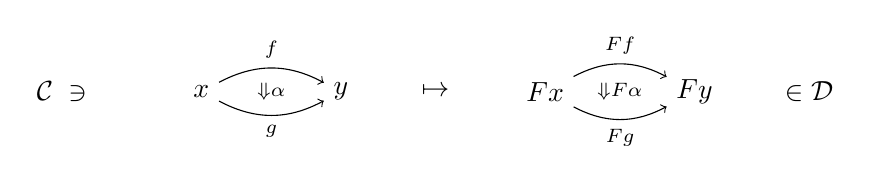
\begin{tikzpicture}[x=1.8em,y=1.5em]
  \node (C)  at (0,0)    {$\mathcal{C}\;\ni$};
  \node (x)  at (2.8,0)  {$x$};
  \node (y)  at (5.6,0)  {$y$};
  \node (mp) at (7.5,0)  {$\mapsto$};
  \node (Fx) at (9.7,0)  {$Fx$};
  \node (Fy) at (12.7,0) {$Fy$};
  \node (D)  at (15.0,0) {$\in\mathcal{D}$};
  \draw[->] (x) to[bend left=28] node[above]{$\scriptstyle f$} (y);
  \draw[->] (x) to[bend right=28] node[below]{$\scriptstyle g$} (y);
  \node at (4.2,0) {$\scriptstyle\Downarrow\alpha$};
  \draw[->] (Fx) to[bend left=28] node[above]{$\scriptstyle Ff$} (Fy);
  \draw[->] (Fx) to[bend right=28] node[below]{$\scriptstyle Fg$} (Fy);
  \node at (11.2,0) {$\scriptstyle\Downarrow F\alpha$};
\end{tikzpicture}
\end{center}
  它保持 0-\trCell{}与 1-\trCell{}的源与目标，并且对水平复合与竖直复合以及
  水平单位与竖直单位都是函子式的。
\end{itemize}
\end{definition}

\begin{definition}\label{def:two-natural-transformation}
介于一对平行 2-\trFunctor{} $F$ 与 $G$ 之间的一个%
\textbf{2-\trNaturalTransformation}（2-natural transformation）
\hTwoCell{\mathcal{C}}{\mathcal{D}}{F}{\Downarrow\phi}{G}
由 $\mathcal{D}$ 中一族 1-\trCell{}
$(\phi_{c}\colon Fc\to Gc)_{c\in\mathcal{C}}$ 给出，后者由 $\mathcal{C}$ 的诸
对象加标，且对 $\mathcal{C}$ 中的诸 1-\trCell{} $f\colon x\to y$ 自然，意即
方块
\begin{center}
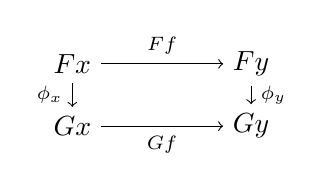
\begin{tikzpicture}[x=1.9em,y=1.5em]
  \node (tl) at (0,1.5) {$Fx$};
  \node (tr) at (3.4,1.5) {$Fy$};
  \node (bl) at (0,0) {$Gx$};
  \node (br) at (3.4,0) {$Gy$};
  \draw[->] (tl) -- node[above]{$\scriptstyle Ff$} (tr);
  \draw[->] (tl) -- node[left]{$\scriptstyle\phi_{x}$} (bl);
  \draw[->] (tr) -- node[right]{$\scriptstyle\phi_{y}$} (br);
  \draw[->] (bl) -- node[below]{$\scriptstyle Gf$} (br);
\end{tikzpicture}
\end{center}
在 $\mathcal{D}$ 中交换，并且对 $\mathcal{C}$ 中的诸 2-\trCell{}
\hTwoCell{x}{y}{f}{\Downarrow\alpha}{g}
也自然，意即诸须状复合 $\phi_{y}\cdot F\alpha$ 与
$G\alpha\cdot\phi_{x}$ 相等：
\begin{center}
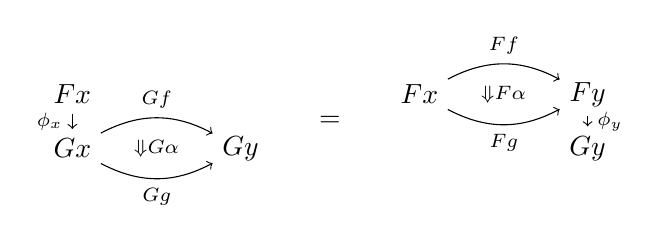
\begin{tikzpicture}[x=1.9em,y=1.5em]
  \node (LFX) at (0,1.3) {$Fx$};
  \node (LGX) at (0,0) {$Gx$};
  \node (LGY) at (3.2,0) {$Gy$};
  \draw[->] (LFX) -- node[left]{$\scriptstyle\phi_{x}$} (LGX);
  \draw[->] (LGX) to[bend left=28] node[above]{$\scriptstyle Gf$} (LGY);
  \draw[->] (LGX) to[bend right=28] node[below]{$\scriptstyle Gg$} (LGY);
  \node at (1.6,0) {$\scriptstyle\Downarrow G\alpha$};
  \node at (4.9,0.65) {$=$};
  \node (RFX) at (6.6,1.3) {$Fx$};
  \node (RFY) at (9.8,1.3) {$Fy$};
  \node (RGY) at (9.8,0) {$Gy$};
  \draw[->] (RFX) to[bend left=28] node[above]{$\scriptstyle Ff$} (RFY);
  \draw[->] (RFX) to[bend right=28] node[below]{$\scriptstyle Fg$} (RFY);
  \node at (8.2,1.3) {$\scriptstyle\Downarrow F\alpha$};
  \draw[->] (RFY) -- node[right]{$\scriptstyle\phi_{y}$} (RGY);
\end{tikzpicture}
\end{center}
\end{definition}

2-\trCategory{}之间的 $3$ 维态射居于 $\Cat$-富集\trCategory{}论的视野之外：

\begin{definition}\label{def:modification}
介于一对平行的 2-\trNaturalTransformation{}之间的一个\textbf{\trModification}
（modification）$\Xi\colon\phi\Rightarrow\psi$
\begin{center}
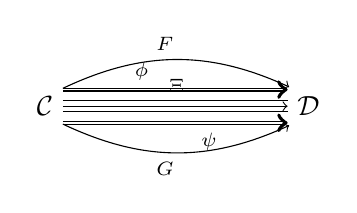
\begin{tikzpicture}[x=1.7em,y=1.5em]
  \node (C) at (0,0) {$\mathcal{C}$};
  \node (D) at (5.6,0) {$\mathcal{D}$};
  \draw[->] (C.45) to[bend left=25] node[above,pos=0.45]{$\scriptstyle F$}
    (D.135);
  \draw[->,double] ([yshift=0.6em]C.east) --
    node[above,pos=0.35]{$\scriptstyle\phi$} ([yshift=0.6em]D.west);
  \draw[->] (C.east) -- (D.west);
  \draw ([yshift=0.2em]C.east) -- ([yshift=0.2em]D.west);
  \draw ([yshift=-0.2em]C.east) -- ([yshift=-0.2em]D.west);
  \node at (2.8,0.5) {$\scriptstyle\Xi$};
  \draw[->,double] ([yshift=-0.6em]C.east) --
    node[below,pos=0.65]{$\scriptstyle\psi$} ([yshift=-0.6em]D.west);
  \draw[->] (C.-45) to[bend right=25] node[below,pos=0.45]{$\scriptstyle G$}
    (D.-135);
\end{tikzpicture}
\end{center}
由 $\mathcal{D}$ 中的如下一族 2-\trCell{}给出：
\begin{center}
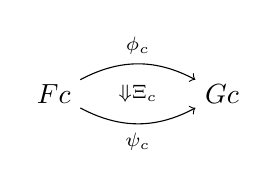
\begin{tikzpicture}[x=1.9em,y=1.5em]
  \node (a) at (0,0) {$Fc$};
  \node (b) at (3.2,0) {$Gc$};
  \draw[->] (a) to[bend left=28] node[above]{$\scriptstyle\phi_{c}$} (b);
  \draw[->] (a) to[bend right=28] node[below]{$\scriptstyle\psi_{c}$} (b);
  \node at (1.6,0) {$\scriptstyle\Downarrow\Xi_{c}$};
\end{tikzpicture}
\end{center}
其由诸对象 $c\in\mathcal{C}$ 加标，且具有如下性质：对 $\mathcal{C}$ 中的任何
1-\trCell{} $f\colon x\to y$，诸须状复合 $\Xi_{y}\cdot Ff$ 与
$Gf\cdot\Xi_{x}$ 在 $\mathcal{D}$ 中相等；并且对 $\mathcal{C}$ 中的任何
2-\trCell{} $\alpha\colon f\Rightarrow g$\footnote{原书印作「$\mathcal{D}$ 中
的任何 2-\trCell{} $\alpha\colon f\Rightarrow g$」。据下方显示式中出现的
$F\alpha$ 与 $G\alpha$，该 2-\trCell{}应居于域 2-\trCategory{} $\mathcal{C}$
之中，疑为「$\mathcal{C}$」之误，此处径改。——译者注}，诸水平复合在
$\mathcal{D}$ 中相等：
\begin{center}
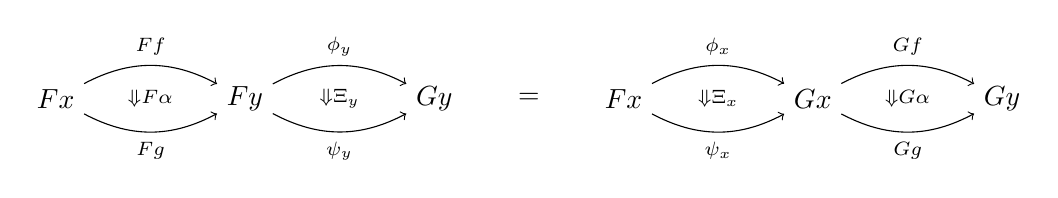
\begin{tikzpicture}[x=1.9em,y=1.5em]
  \node (Fx1) at (0,0) {$Fx$};
  \node (Fy1) at (3.6,0) {$Fy$};
  \node (Gy1) at (7.2,0) {$Gy$};
  \node (eq)  at (9.0,0) {$=$};
  \node (Fx2) at (10.8,0) {$Fx$};
  \node (Gx2) at (14.4,0) {$Gx$};
  \node (Gy2) at (18.0,0) {$Gy$};
  \draw[->] (Fx1) to[bend left=28] node[above]{$\scriptstyle Ff$} (Fy1);
  \draw[->] (Fx1) to[bend right=28] node[below]{$\scriptstyle Fg$} (Fy1);
  \node at (1.8,0) {$\scriptstyle\Downarrow F\alpha$};
  \draw[->] (Fy1) to[bend left=28] node[above]{$\scriptstyle\phi_{y}$} (Gy1);
  \draw[->] (Fy1) to[bend right=28] node[below]{$\scriptstyle\psi_{y}$} (Gy1);
  \node at (5.4,0) {$\scriptstyle\Downarrow\Xi_{y}$};
  \draw[->] (Fx2) to[bend left=28] node[above]{$\scriptstyle\phi_{x}$} (Gx2);
  \draw[->] (Fx2) to[bend right=28] node[below]{$\scriptstyle\psi_{x}$} (Gx2);
  \node at (12.6,0) {$\scriptstyle\Downarrow\Xi_{x}$};
  \draw[->] (Gx2) to[bend left=28] node[above]{$\scriptstyle Gf$} (Gy2);
  \draw[->] (Gx2) to[bend right=28] node[below]{$\scriptstyle Gg$} (Gy2);
  \node at (16.2,0) {$\scriptstyle\Downarrow G\alpha$};
\end{tikzpicture}
\end{center}
\end{definition}

由 2-\trCategory{}组成的\trCategory{}是\trCartesianClosed，其\trInternalHom{}
$\mathcal{B}^{\mathcal{A}}$ 定义为由 2-\trFunctor、2-\trNaturalTransformation{}%
与\trModification{}组成的 2-\trCategory。于是，我们现在可以把一个\textbf{3-\trCategory}定义为
富集于 2-\trCategory{}之上的一个\trCategory。

\begin{corollary}\label{cor:two-cat-three-category}
存在一个由 2-\trCategory、2-\trFunctor、2-\trNaturalTransformation{}与\trModification{}组成
的 3-\trCategory{} $2\text{-}\mathit{Cat}$。
\end{corollary}

\begin{proof}
\cref{lem:cartesian-closed-v-category}证明了：任何\trCartesianClosed{}%
\trCategory{}都富集于其自身之上。于是，$2\text{-}\mathit{Cat}$ 定义一个
3-\trCategory。
\end{proof}

\subsection*{练习}

\begin{exercise}\label{ex:relate-two-category-structures}
在富集之基为 $\Cat$ 的情形下，将\cref{def:two-functor}与%
\cref{def:two-natural-transformation}中逐项列出的诸结构，同附录 A 中的%
\cref{def:v-enriched-functor}与\cref{def:vnatural-transformation}中逐项列出的
诸结构联系起来。
\end{exercise}

\begin{exercise}\label{ex:unpack-3-category-definition}
对于拥有大块书写面的读者，请展开刚刚给出的 3-\trCategory{}的定义。
\end{exercise}

\begin{exercise}\label{ex:involutive-op-and-duals}
\begin{enumerate}[label=(\roman*)]
\item 证明：把一个 1-\trCategory{}送到其反者的那支\trFunctor{}定义一支对合
  2-\trFunctor{} $(-)^{\mathrm{op}}\colon\Cat^{\mathrm{co}}\to\Cat$，作用于由%
  \trCategory、\trFunctor{}与\trNaturalTransformation{}组成的 2-\trCategory{}%
  之上。
\item 类似地，把一个 2-\trCategory{}送到其三个对偶之一的那些\trFunctor{}可以
  被理解为由 2-\trCategory、2-\trFunctor、2-\trNaturalTransformation{}与%
  \trModification{}组成的 3-\trCategory{}的诸对合。这些映射各自具有何种变异性？
\end{enumerate}
\end{exercise}

